\documentclass[a4paper]{article}

\usepackage[portuguese]{babel}
\usepackage{comment}
\usepackage[T1]{fontenc}
\usepackage[utf8]{inputenc}
\usepackage{hyperref}
\usepackage{graphicx}
\usepackage{float}
\usepackage{multirow}
\usepackage[hypcap]{caption} % makes \ref point to top of figures and tables
\usepackage{amsmath}
\usepackage{multicol} %for page layout on section Maximização do Throughput
%\usepackage[usenames,dvipsnames,svgnames,table]{xcolor}
\usepackage{pdflscape}	% landscape pages
\usepackage{subcaption}

\begin{document}

\begin{titlepage}

\begin{center}


\includegraphics[width=6cm]{./title}\\[3cm]

\textsc{\LARGE Projecto de Sistemas Digitais}\\[1.5cm]

\textsc{\Large Laboratório 2}\\[1.5cm]


{ \huge \bfseries Escalonamento e Partilha de Recursos \\[3cm] }


\noindent
\begin{minipage}{0.4\textwidth}
\begin{flushleft} \large
Rafael Gonçalves, 73786
\end{flushleft}
\end{minipage}
\begin{minipage}{0.4\textwidth}
\begin{flushright} \large
Gonçalo Ribeiro, 73294
\end{flushright}
\end{minipage}

\vfill

{\large \today}


\end{center}

\end{titlepage}

\tableofcontents
\pagebreak

\section{Introdução}
O presente trabalho tem por objectivo o desenho e implementação de um processador dedicado para processamento morfológico de imagens binárias i.e.\ imagens cujos pixeis podem ter apenas dois valores distintos.

As operações a realizar sobre as imagens são cinco: erosão, dilatação, fecho (dilatação seguida de erosão), abertura (erosão seguida de dilatação) e extração de contornos (diferença entre a imagem original e a sua erosão).

O elemento estruturante considerado é um quadrado de $3\times3$ pixeis---por exemplo na operação de erosão analisa-se uma área $3\times3$ px centrada nesse pixel para decidir se o mesmo deve ser erodido.

As imagens consideradas têm no máximo $128\times128$ px. Uma imagem é transferida de um computador para a uma BRAM da FPGA via USB e o processador dedicado deve ler dessa BRAM de entrada e escrever a imagem transformada numa BRAM de saída. A imagem transformada é depois transferida de volta PC, onde pode ser visualizada.

O desempenho do circuito é avaliado pelo tempo de processamento dos dados entre as duas memórias.

\section{Formato das Imagens}
O formato das imagens não é definido no enunciado do projecto. É esperado que os alunos desenvolvam um formato de imagem que julguem mais adequado.

As imagens têm no máximo $128\times128\times1$ bits (2 kB), que é precisamente a dimensão de cada uma das 4 BRAMs existentes na FPGA XC3S-100E-4CP132. Como tal no caso das imagens maiores a BRAM de entrada é completamente preenchida, o que significa que não sobram bits para representar por exemplo as dimensões da imagem. Assim, essa informação não pode fazer parte do formato da imagem.

Decidiu-se então que as dimensões da imagem (largura e altura) são passadas ao processador dedicado fazendo uso dos 8 interruptores existentes na placa de desenvolvimento. Introduz-se primeiro a largura e pressiona-se um botão de pressão para armazenar essa dimensão. De seguida faz-se o mesmo para a altura.

A imagem é representada em memória sempre como 4 palavras de 32 bits por cada linha da imagem. Se a imagem tiver menos que 128 bits de largura é introduzido \textit{padding} que perfaça 128 bits. O \textit{padding} utilizado consiste na extensão do último bit válido de cada linha da imagem. Estas características foram escolhida de forma a facilitar o processamento da imagem.

\section{Arquitectura}
% intro à arquitectura
As operações elementares (dilatação e erosão) podem ser realizadas em dois passos distintos: primeiro executa-se a operação apenas na horizontal, i.e. usando um elemento estruturante de dimensão $3\times1$; de seguida expande-se o resultado para a linha acima e para abaixo.

A arquitectura projectada faz uso desta propriedade e como tal tem duas datapaths pricipais. A primeira, que realiza alterações apenas na horizontal, é designada por \textit{Horizontal Alteration after Line Fetch} (HALF). A segunda faz a expansão vertical e chama-se \textit{Storing Alterations after Vertical Exchange} (SAVE). Cada uma destas datapahts tem uma FSM respectiva. A \autoref{fig:poc} ilustra as duas fases de processamento.

\begin{figure}[h]
	\centering
	\begin{subfigure}[b]{0.32\textwidth}
		\centering
		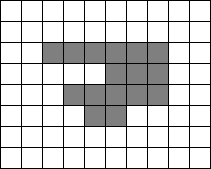
\includegraphics[width=\linewidth]{poc_orig}
		\caption{}
		\label{fig:por_orig}
	\end{subfigure}
	\begin{subfigure}[b]{0.32\textwidth}
		\centering
		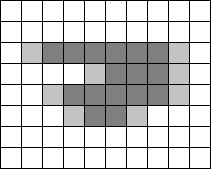
\includegraphics[width=\linewidth]{poc_HALF}
		\caption{}
		\label{fig:poc_HALF}
	\end{subfigure}
	\begin{subfigure}[b]{0.32\textwidth}
		\centering
		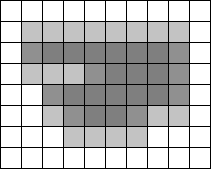
\includegraphics[width=\linewidth]{poc_SAVE}
		\caption{}
		\label{fig:poc_SAVE}
	\end{subfigure}
	\caption{imagem (a) original (b) após HALF (c) após HALF e SAVE}
	\label{fig:poc}
\end{figure}

Para além dessas duas componentes principais do circuito existe ainda outra que é responsável por fazer o \textit{padding} de cada linha antes do armazenamento na BRAM de saída.

\subsection{HALF}
% intro ao HALF
HALF é responsável por fazer as transformações horizontais de cada linha da imagem, como exemplificado na \autoref{fig:poc_HALF}.

\subsubsection{Datapath}
A datapath da HALF tem por base dois módulos: um bloco de dilatação (D) e outro de erosão (E). Uma dilatação horizontal corresponde basicamente a fazer um OR de cada bit com o bit à sua esquerda e à sua direita; da mesma forma uma erosão corresponde a um AND. Assim, os blocos D e E são \textit{arrays} dessas portas de forma a processar palavras 32 bits de cada vez. Existe, naturalmente, alguma lógica extra que é responsável por expansões de uma palavra para outra---por exemplo se uma imagem tiver como largura duas palavras de 32 bits a dilatação horizontal da primeira pode afectar o primeiro bit da segunda; e o primeiro bit da segunda pode afectar o último bit da primeira. O circuito dos blocos D e E pode ver-se na \autoref{fig:HALF_E_D_blocks}.

\begin{figure}[h]
	\centering
	\begin{subfigure}[b]{0.45\textwidth}
		\centering
		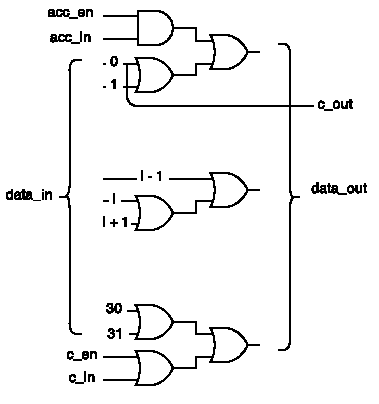
\includegraphics[width=\linewidth]{HALF_D_block}
		\caption{}
		\label{fig:HALF_D_block}
	\end{subfigure}
	\begin{subfigure}[b]{0.45\textwidth}
		\centering
		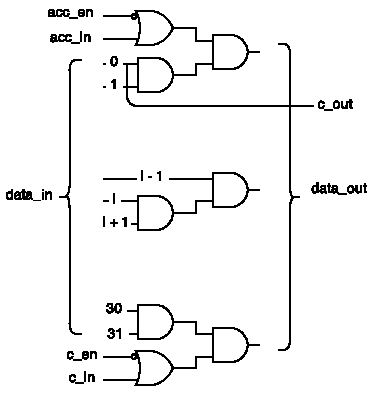
\includegraphics[width=\linewidth]{HALF_E_block}
		\caption{}
		\label{fig:HALF_E_block}
	\end{subfigure}
	\caption{(a) bloco de dilatação (b) bloco de erosão}
	\label{fig:HALF_E_D_blocks}
\end{figure}

%explicar carry e accum
A entrada \texttt{c\_in} permite que o MSB (\textit{most significant bit}) de uma palavra seja alterado tendo em conta o LSB (\textit{least significant bit}) da palabra anterior. Por outro lado, a entrada \texttt{acc\_in} permite que o LSB de uma palavra seja alterado tomando em consideração o MSB da palavra seguinte. As entradas \texttt{c\_en} e \texttt{acc\_en} permitem indicar se tanto \texttt{c\_in} como \texttt{acc\_in} têm valores válidos. Na primeira palavra de cada imagem \texttt{c\_en} deve estar a \texttt{0} e na última palavra \texttt{acc\_en} deve estar a \texttt{0}. Nos restantes casos esses sinais devem estar a \texttt{1}.

Poder usar o sinal \texttt{acc\_in} significa necessariamente que quando uma palavra é processada por um dos blocos da \autoref{fig:HALF_E_D_blocks} a palavra seguinte já tem que ser sido lida da memória. Para isso existe na arquitectura um registo \texttt{\_accum} para cada bloco. Este registo permite pôr a palavra $n$ em espera até que a palavra $n+1$ seja lida. Quando a palavra $n+1$ é lida tem-se toda a informação necessária ao processamento da palavra $n$. O mesmo registo põe em espera o \textit{c\_out} da palavra $n-1$ para que possa ser usado no processamento da $n$. Estes registos podem ser vistos na \autoref{fig:HALF_datapath}.

Outra particularidade da datapath da HALF é que para realizar as operações compostas o output das operações elementares pode ser redireccionado para a entrada do bloco complementar. Assim um fecho horizontal pode ser calculado passando \texttt{data\_in} pelo bloco D e redireccionando o output para a entrada do bloco E. À saída teremos o fecho horizontal da palavra em \texttt{data\_in}.

Para que o redireccionamento de uma palavra de um bloco para outro não aumentasse não criasse um caminho crítico dentro do bloco introduziu-se um registo \texttt{\_delay\_reg} à saída dos blocos D e E. Estes registos permitem que nas operações de abertura e fecho se faça armazenamento do resultado intermédio para que o caminho crítico não possa ser o percurso desde \texttt{data\_in} até ao \texttt{data\_out} do segundo bloco.

Devido aos atrasos causados pelos registos \texttt{\_accum} e \texttt{\_delay\_reg} é necessário fazer uma compensação---i.e.\ um atraso---dos sinais de controlo da datapath. Para isso os sinais de controlo \texttt{\_carry\_en} e \texttt{\_accum\_en} são passados por um ou dois registos, conforme se trate, respectivamente, de uma operação elementar ou de uma composta. Esse atraso variável é controlado pelos sinais \texttt{\_delay}.

Paralelamente à saída \texttt{output\_func} existe também a \textit{bus} \texttt{output\_orig} que é a palavra original correspondente à palavra transformada durante a HALF. A palavra original é usada apenas durante a SAVE e somente no caso da operação de extracção de contornos. A palavra original é atrasada fazendo uso do registo \texttt{d\_accum\_en}, que não é usado para outro fim durante extracções de contornos. Assim, a palavra original e transformada saem da datapath sincronizadas.

O diagrama da datapath da HALF está patente na \autoref{fig:HALF_datapath}.

\begin{figure}[H]
	\centerline{
		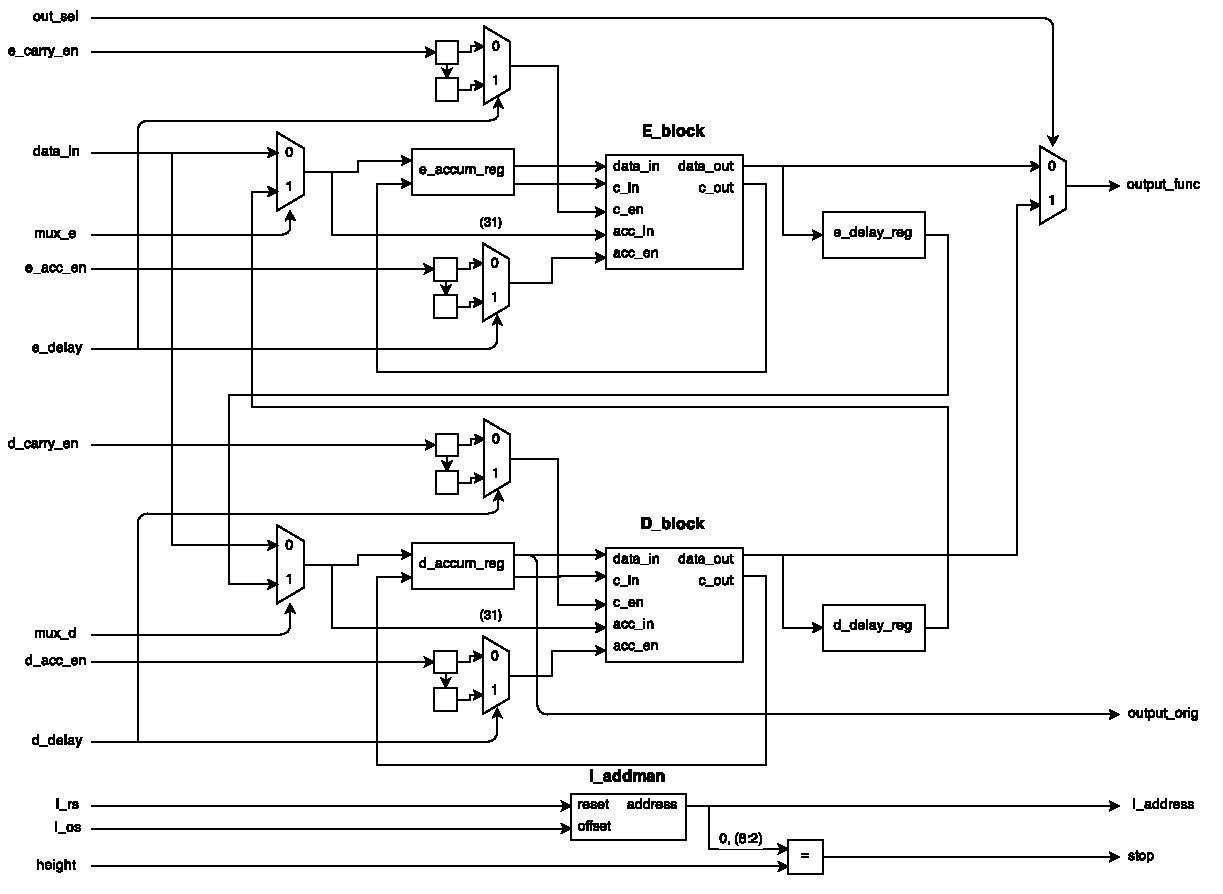
\includegraphics[width=.95\paperwidth]{HALF_datapath}
	}
	\caption{datapath da HALF}
	\label{fig:HALF_datapath}
\end{figure}

O bloco \texttt{i\_addman} é o \textit{address manager} da BRAM de entrada. Este bloco é um contador que regista qual o endereço a ser lido da BRAM de entrada. Com base no endereço actual e na altura da imagem é possível calcular o sinal \texttt{stop}, que indica à FSM se o trabalho da HALF terminou.

\subsubsection{FSM}
A máquina de estados da HALF pode ser vista na \autoref{fig:HALF_FSM}.

\begin{figure}
	\centering
	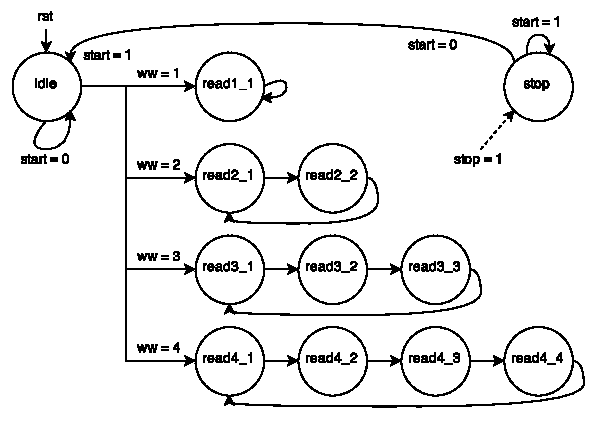
\includegraphics[width=0.8\linewidth]{HALF_FSM}
	\caption{máquina de estados da HALF}
	\label{fig:HALF_FSM}
\end{figure}

Existem duas classes de outputs nesta máquina de estados: uns dependem apenas do estado actual, sendo independentes do tipo de operação; os outros dependem apenas do tipo de operação.

Da primeira classe fazem parte os \textit{enables} dos blocos D e E, reset do \texttt{addman}, offset da BRAM de entrada e o offset da unidade de armazenamento do SAVE.

Da outra classe fazem parte os sinais de controlo de multiplexers e os sinais de \textit{delay}.

%\begin{table}
%\small
%\centerline{
%\begin{tabular}{|c||c|c|c|c|c|c|c|c|c|c|c|c|}
%\hline 
%& idle & read1\_1 & read2\_1 & read2\_2 & read3\_1 & read3\_2 & read3\_3 & read4\_1 & read4\_2 & read4\_3 & read4\_4 & stop\\ 
%\hline 
%\hline
%mux\_e & • & • & • & • & • & • & • & • & • & • & • & • \\ 
%\hline 
%mux\_d & • & • & • & • & • & • & • & • & • & • & • & • \\ 
%\hline 
%e\_carry\_en & • & • & • & • & • & • & • & • & • & • & • & • \\ 
%\hline 
%d\_carry\_en & • & • & • & • & • & • & • & • & • & • & • & • \\ 
%\hline 
%e\_acc\_en & • & • & • & • & • & • & • & • & • & • & • & • \\ 
%\hline 
%d\_acc\_en & • & • & • & • & • & • & • & • & • & • & • & • \\ 
%\hline 
%e\_delay & • & • & • & • & • & • & • & • & • & • & • & • \\ 
%\hline 
%d\_delay & • & • & • & • & • & • & • & • & • & • & • & • \\ 
%\hline 
%i\_rs & • & • & • & • & • & • & • & • & • & • & • & • \\ 
%\hline
%i\_en & • & • & • & • & • & • & • & • & • & • & • & • \\ 
%\hline 
%i\_os & • & • & • & • & • & • & • & • & • & • & • & • \\ 
%\hline 
%f\_os & • & • & • & • & • & • & • & • & • & • & • & • \\ 
%\hline 
%\end{tabular}
%}
%\caption{sinais de saída da FSM para cada estado}
%\label{tab:HALF_FSM_outputs}
%\end{table}

\subsection{SAVE}
% intro ao SAVE

O módulo SAVE recebe a imagem já processada horizontalmente, e procede à sua ``expansão'' na vertical. Para isto precisa de três palavras (correspondentes às linhas actual, anterior e seguinte).

\subsubsection{Datapath}

% Falta aqui a unidade de armazenamento

Uma vez disponíveis as três palavras relevantes (ou duas, no caso da primeira e última palavra, que não têm antecessor nem sucessor, respectivamente), são sobre si efectuadas as operações lógicas correspondentes à operação morfológica a realizar sobre a imagem (ver \autoref{fig:SAVE_datapath_E_D}).

\begin{figure}[h]
	\centering
	\begin{subfigure}[b]{0.45\textwidth}
		\centering
		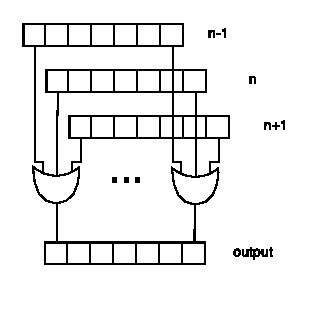
\includegraphics[width=\linewidth]{SAVE_datapath_D}
		\caption{Dilatação}
		\label{fig:SAVE_datapath_D}
	\end{subfigure}
	\begin{subfigure}[b]{0.45\textwidth}
		\centering
		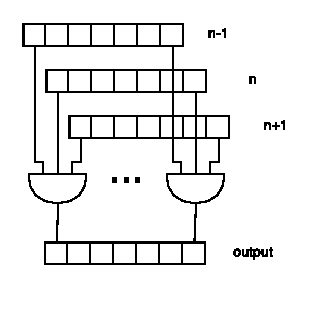
\includegraphics[width=\linewidth]{SAVE_datapath_E}
		\caption{Erosão}
		\label{fig:SAVE_datapath_E}
	\end{subfigure}
	\caption{Unidades funcionais da Datapath do SAVE}
	\label{fig:SAVE_datapath_E_D}
\end{figure}

Estes blocos são dispostos na arquitectura especificada na \autoref{fig:SAVE_Datapath}, de maneira a realizar as várias operações.

Caso a operação seja simples, o resultado do módulo HALF é direccionado para a unidade de armazenamento principal, e a sua saída para os blocos lógicos, cujo resultado vai para a saída.

No caso de ser uma operação composta (abertura ou fecho), a saída da primeira operação é redireccionada para uma segunda unidade de armazenamento, a partir da qual é realizada a última operação antes do armazenamento na memória.

Finalmente, caso a operação seja detecção de limites, a imagem erodida horizontalmente é direccionada para a unidade de armazenamento principal, e posteriormente erodida verticalmente. Simultaneamente, a imagem original, inalterada, é direccionada para a segunda unidade de armazenamento, cuja saída é direccionada para o bloco de Subtracção, cuja única operação é uma \texttt{XOR} bit-a-bit entre os dois operandos.

\begin{figure}[h]
	\centering
	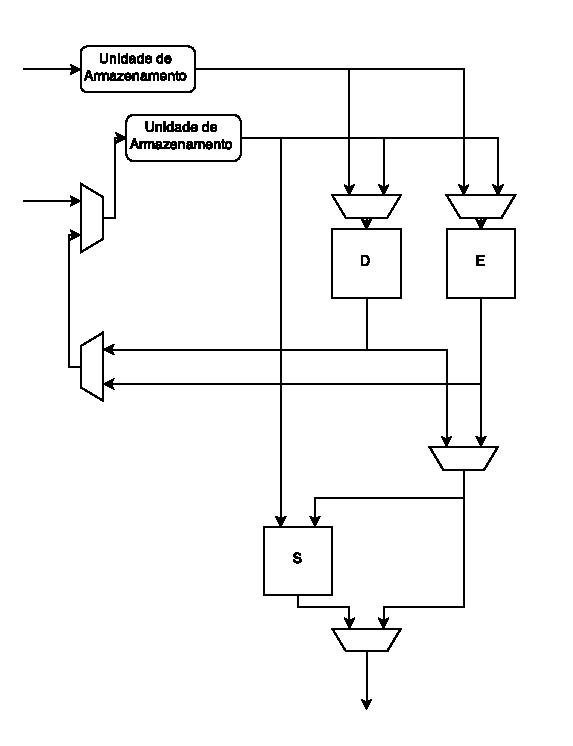
\includegraphics[width=0.6\linewidth]{SAVE_Datapath}
	\caption{Datapath do módulo SAVE}
	\label{fig:SAVE_Datapath}
\end{figure}

\subsubsection{FSM}

\subsection{\textit{Padder}}
% intro ao padder

\subsubsection{Datapath}

\subsubsection{FSM}

\subsection{Interligação dos Componentes}	% titulo melhor ?

\section{\textit{Performance}}	% titulo melhor ?

\section{Conclusões e Comentários}

\end{document}